\section{Prozessverbesserungen \skript{\pageref{sk-chapter-filtern}}}
\subsection{Gewichteter Mittelwert}
	Besitzt man die Möglichkeit Messwerte aus zwei Messsystemen $X_1$ und $X_2$ mit unterschiedlicher Genauigkeit ($var(X_1)$/$var(X_2)$) zu beziehen, so kann man die Messwerte so gewichten, dass eine optimale Genauigkeit besteht.\\
	
	$\boxed{X_{opt} = t\cdot X_1 + (1-t) \cdot X_2} \qquad \rightarrow t$ so wählen, dass $var(X_{opt})$ minimal wird\\


	\hspace*{1cm} $var(X_{opt}) = t^2 \cdot var(X_1) + (1-t)^2 \cdot var(X_2) \qquad \rightarrow$ nach $t$ ableiten und Null setzen \\  
	
	$\Rightarrow \boxed{t = \dfrac{\sigma_2^2}{\sigma_1^2 + \sigma_2^2}} \; ; \; \boxed{1-t = \dfrac{\sigma_1^2}{\sigma_1^2 + \sigma_2^2}}$
	\hspace{1cm} $var(X_{opt}) = \dfrac{\sigma_1^2 \cdot \sigma_2^2}{\sigma_1^2 + \sigma_2^2}$

\subsection{Kalman-Filter}
	\textbf{Prinzip:} bestmögliche Schätzung für Systemzustand auf Grund von fehlerbehafteter
	Messung und Systementwicklung. \\

	\subsubsection{Datenfluss im Kalman-Filter \skript{\pageref{sk-datenfluss}}}
			\begin{tikzpicture}
	% Styles
		[	inner sep = 2mm,
			block/.style={rectangle, minimum size=6mm, thick, draw=blue!50!black!30,
				top color=white, bottom color=blue!50},
			add/.style={circle, minimum size=5mm, thick, draw=white!50!black!50,
				top color=white, bottom color=white!50!black!50, inner sep=1pt},
			point/.style={circle, inner sep=0pt, minimum size=0pt}
		]
	% Graphic
		% Blocks
		\node at (0,0)		(add1)	[add]	{$+$};
		\node at (0,-2)		(phi1)	[block]	{$\varphi_{k-1}$};
		\node at (2,-2)		(del1)	[block]	{\textit{DELAY}};
		\node at (4.5,0)	(h1)	[block]	{$H_k$};
		\node at (6,0)		(add2)	[add]	{$+$};
		\node at (8,0)		(sub1)	[add]	{$-$};
		\node at (9.5,0)	(k1)	[block]	{$K_k$};
		\node at (9.5,-2)	(h2)	[block]	{$H_k$};
		\node at (11,0)		(add3)	[add]	{$+$};
		\node at (12.5,-2)	(phi2)	[block]	{$\varphi_{k-1}$};
		\node at (14.5,-2)	(del2)	[block]	{\textit{DELAY}};
		% Labels
		\node at (0,1)		(uk)			{$u_k$};
		\node at (3.5,0.2)					{$x_k$};
		\node at (6,-1.2)	(wk)			{$w_k$};
		\node at (7,0.2)					{$z_k$};
		\node at (11,-2.4)					{$\hat{x}_{k|k-1}$};
		\node at (17,0)		(xk)			{$\hat{x}_k$};
		
		\node at (13.5, -1) {Vorhersage};
		\node at (9.5, -1) {Korrektur};
		
		% Connection Points
		\node at (3.5,0)	(p1)	[point]	{};
		\node at (3.5,-2)	(p2)	[point]	{};
		\node at (8,-2)		(p3)	[point]	{};
		\node at (11,-2)	(p4)	[point]	{};
		\node at (16,0)		(p5)	[point]	{};
		\node at (16,-2)	(p6)	[point]	{};
		
		% Braces Labels
		\node at (1.5,-3.6)					{System};
		\node at (5.5,-3.6)					{Messung};
		\node at (12,-3.6)					{Kalman-Filter};
	
		% Connectors
		\graph[use existing nodes] {
			uk -> add1 -> h1 -> add2 -> sub1;
			p1 -- p2 -> del1 -> phi1 -> add1;
			wk -> add2;
			sub1 -> k1 -> add3 -> xk;
			p5 -- p6 -> del2 -> phi2 -> h2 -- p3 -> sub1;
			p4 -> add3;
		};
		
		% Braces
		\draw[decoration={brace,amplitude=3mm,mirror},decorate] (-0.5,-3) -- (3.5,-3);
		\draw[decoration={brace,amplitude=3mm,mirror},decorate] (4,-3) -- (7,-3);
		\draw[decoration={brace,amplitude=3mm,mirror},decorate] (7.5,-3) -- (16.5,-3);
		
	\end{tikzpicture}
%		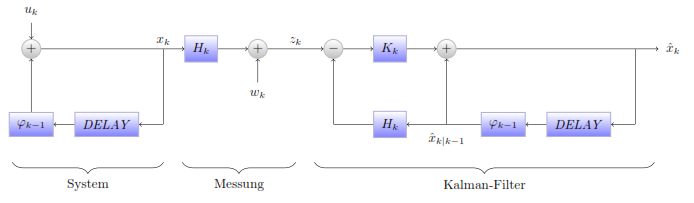
\includegraphics[width=1\textwidth]{./bilder/kalman.png}
	
	\begin{minipage}{8cm}
		\begin{tabular}{ll}
			$u_k$: & Systemungenauigkeiten \\
			$w_k$: & Messfehler \\
			$x_k$: & Unbeobachtete Zustandsvariable \\
			$z_k$: & Fehlerbehaftete Messung von $x_k$ \\
			$\hat{x}_{k|k-1}$: & Vorhersage: $\hat{x}_{k|k-1} = \varphi_{k-1} \hat{x}_{k-1}$\\
			$\hat{x}_k$: & Schätzer für $x_k$ (aus $\hat{x}_{k|k-1}$ und $z_k$)\\
		\end{tabular}
	\end{minipage}
	\begin{minipage}{8cm}
		\begin{tabular}{ll}
			$\varphi_{k-1}$: & Systementwicklung: $x_{k+1}=\varphi_k x_k + u_k$ \\
			$H_k$: & Messung der Zustandsvariablen: $z_k = H_k x_k + w_k$ \\
			$K_k$: & Kalman-Matrix: $\hat{x}_k = (I-K_k H_k)\hat{x}_{k|k-1} + K_k z_k$ \\
		\end{tabular}
	\end{minipage}
	
	\begin{minipage}{8cm}
		$Q_k = E(u_k u_k^t) = \begin{pmatrix} \sigma_1^2 & 0 & \hdots \\
								0 & \sigma_2^2 & \hdots \\
								\vdots & \vdots & \ddots \end{pmatrix}$ \\
		
		$R_k = E(w_k w_k^t) = \begin{pmatrix} \rho_1^2 & 0 & \hdots \\
								0 & \rho_2^2 & \hdots \\
								\vdots & \vdots & \ddots \end{pmatrix}$ \\
		
		$P_k = E(\tilde{x}_k \tilde{x}_k^t) = \begin{pmatrix} 
							\tilde{x}_{k,1}^2 & \tilde{x}_{k,1}\tilde{x}_{k,2} & \hdots \\
							\tilde{x}_{k,2}\tilde{x}_{k,1} & \tilde{x}_{k,2}^2 & \hdots \\
							\vdots & \vdots & \ddots 	\end{pmatrix}$ 
	\end{minipage}
	\begin{minipage}{8cm}
		\begin{tabular}{ll}
				$Q_k$: & Systemfehler-Kovarianzmatrix \\
				$u_k$: & Systemungenauigkeiten \\
				$\sigma_i$: & Varianz der Systemungenauigkeiten \\
				$R_k$: & Messfehler-Kovarianzmatrix \\
				$w_k$: & Messfehler \\
				$\rho_i$: & Varianz der Messungen \\
				$P_k$: & Schätzfehler-Kovarianzmatrix \\
				$\tilde{x}_k$: & Schätzfehler: $\tilde{x}_k=\hat{x}_k-x_k$ \\
		\end{tabular}
	\end{minipage}

\newpage
	
	\subsubsection{Vorgehen}
	\begin{enumerate}
		\item Bestimmung des Zustandsvektors $x_k$ und des Messvektors $z_k$
		\item Aufstellen der Messmatrix $H_k$ aus: $z_k = H_k x_k$
		\item Berechnen der Systementwicklung $\varphi_k$ damit $x_{k+1}=\varphi_k x_k$
		\item Aufstellen der Fehler-Kovarianzmatrixen $Q_k$ und $R_k$
		\item \textbf{Vorhersage-Schritt:} \hspace{1cm}\fbox{
									$\hat{x}_{k+1|k} = \varphi_k \hat{x}_k  \qquad
								   P_{k+1|k} = \varphi_k P_k \varphi_k^t +Q_k$ }
		\item \textbf{Korrektur-Schritt:} \hspace{1cm}\fbox{
									$\hat{x}_k = (I-K_kH_k)\hat{x}_{k|k-1} + K_k z_k \qquad
									 P_k = (I-K_kH_k)P_{k|k-1}(I-K_kH_k)^t + K_kR_kK_k^t$ }
		\item \textbf{Bestimmung des optimalen $K_k$:} \hspace{1cm}\fbox{
									$K_k = P_{k|k-1}H_k^t(H_kP_{k|k-1}H_k^t + R_k)^{-1}$}
		\item Damit wird $P_k$ vereinfacht zu: $P_k = (I-K_kH_k) P_{k|k-1}$ \hspace{1cm} 
		$ \rightarrow P_k$ bleibt variabel
	\end{enumerate}
	
	\subsubsection{Vereinfachung}
		In der Praxis kann meist davon ausgegangen werden, dass $\varphi_k$, $R_k$,
		$Q_k$ und $H_k$ konstant sind. Damit werden auch $P_k$ und $K_k$ konstant und
		die Vorhersage wird vereinfacht zu: $\hat{x}_k = \hat{x}_{k|k-1} 
		+ K(z_k-H\hat{x}_{k|k-1})$ \\